\section*{Задание 1}
Создать базу знаний: «ПРЕДКИ», позволяющую наиболее эффективным способом (за меньшее количество шагов, что обеспечивается меньшим количеством предложений БЗ - правил), и используя разные варианты (примеры) одного вопроса, определить (указать: какой вопрос для какого варианта):
\begin{enumerate}
	\item по имени субъекта определить всех его бабушек (предки 2-го колена),
	\item по имени субъекта определить всех его дедушек (предки 2-го колена),
	\item по имени субъекта определить всех его бабушек и дедушек (предки 2-го
	колена),
	\item по имени субъекта определить его бабушку по материнской линии (предки 2-го колена),
	\item по имени субъекта определить его бабушку и дедушку по материнской линии (предки 2-го колена).
\end{enumerate}
Минимизировать количество правил и количество вариантов вопросов. Использовать конъюнктивные правила и простой вопрос.

\begin{lstinputlisting}[label=third,caption=Решение задания №1, language=prolog, firstline=1, lastline=28]{../lab_14.pro}
\end{lstinputlisting}

\begin{figure}[H]
	\caption{Таблица к заданию.}
	\begin{center}
		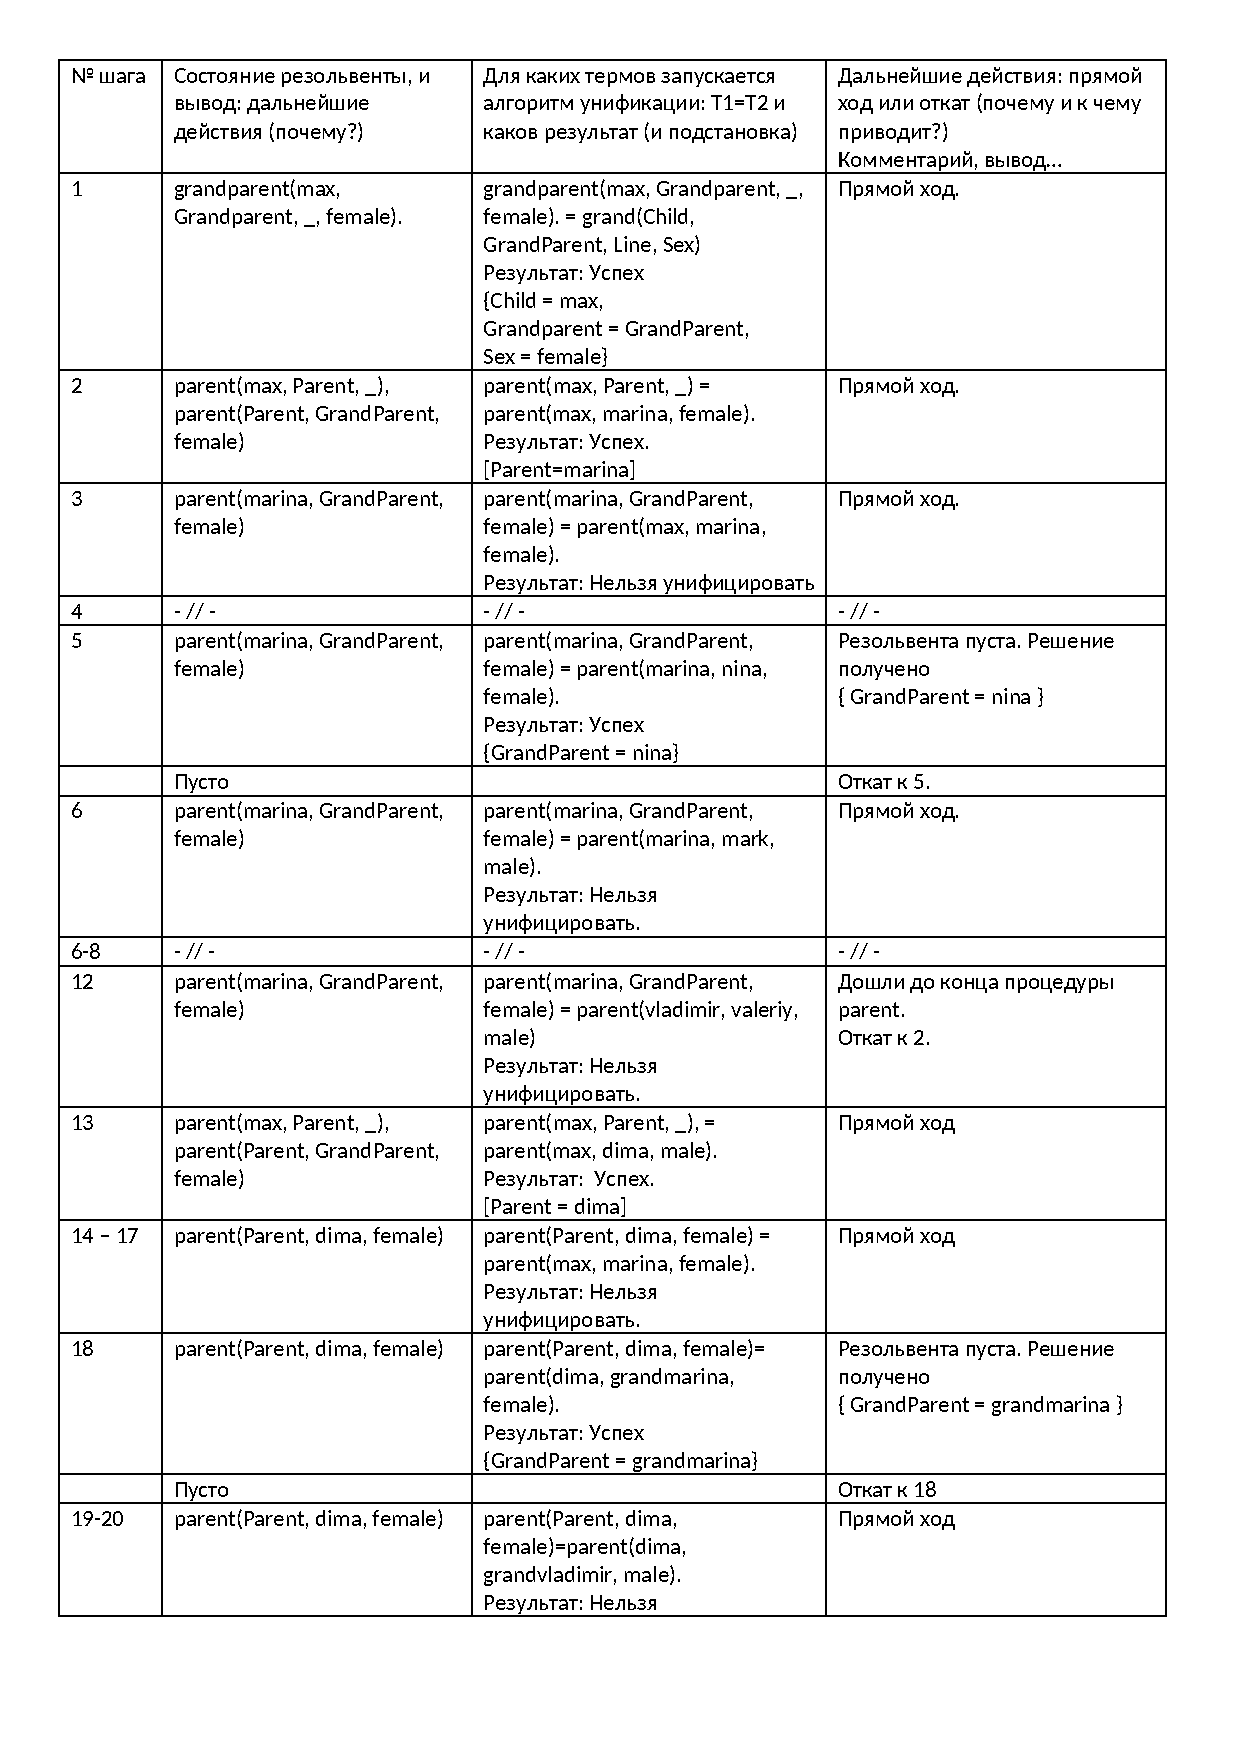
\includegraphics[scale=0.85]{img/14.1.pdf}
	\end{center}
	
\end{figure}

\begin{figure}[H]
	\begin{center}
		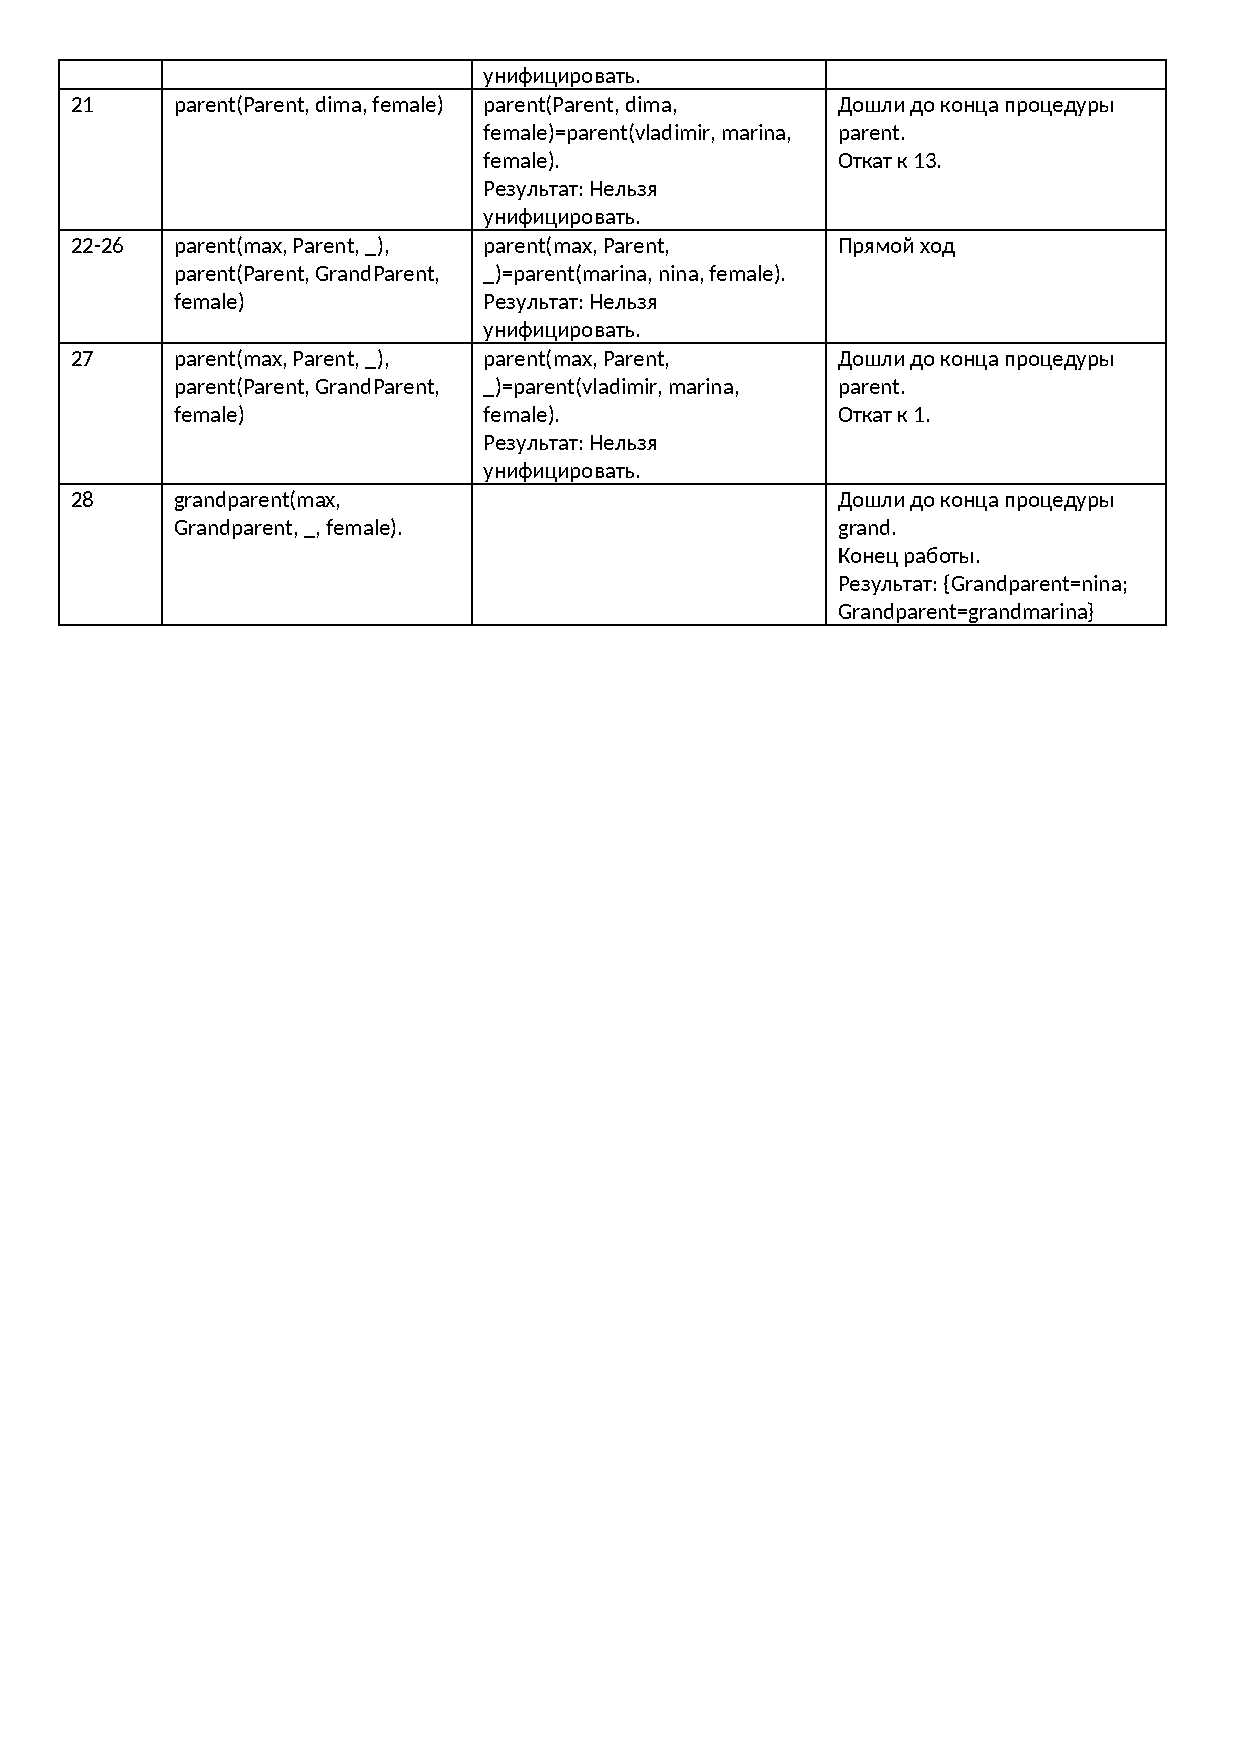
\includegraphics[scale=0.85]{img/14.2.pdf}
	\end{center}
	
\end{figure}